\documentclass[11pt]{article}
\usepackage[utf8]{inputenc}
\usepackage[dvips]{graphicx}
\usepackage{fancybox}
\usepackage{verbatim}
\usepackage{multirow,array}
\usepackage{latexsym}
\usepackage{alltt}
\usepackage{hyperref}
\usepackage{textcomp}
\usepackage{color}
\usepackage{amsmath}
\usepackage{amsfonts}
\usepackage{tikz}
\usepackage{float}
\usepackage[hmargin=3cm,vmargin=5.0cm]{geometry}
%\topmargin=0cm
\topmargin=-2cm
\addtolength{\textheight}{6.5cm}
\addtolength{\textwidth}{2.0cm}
%\setlength{\leftmargin}{-5cm}
\setlength{\oddsidemargin}{0.0cm}
\setlength{\evensidemargin}{0.0cm}


\begin{document}

\section*{How to draw graphs - examples} 
By using these examples you can easily draw graphs and trees in the answer sheet.
\begin{figure}[H]
	\centering
	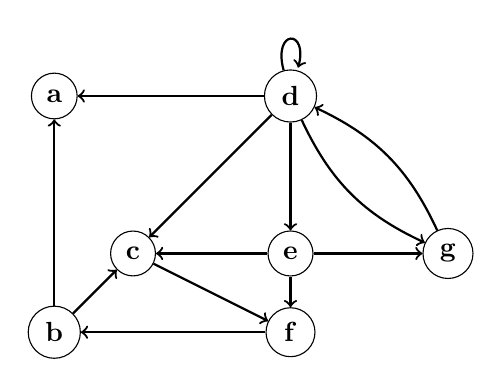
\begin{tikzpicture}
	
	\node[shape=circle,draw=black] (a) at (0, 3)     {\textbf{a}};
	\node[shape=circle,draw=black] (b) at (0, 0)     {\textbf{b}};
	\node[shape=circle,draw=black] (c) at (1, 1)     {\textbf{c}};
	\node[shape=circle,draw=black] (d) at (3, 3)     {\textbf{d}};
	\node[shape=circle,draw=black] (e) at (3, 1)     {\textbf{e}};
	\node[shape=circle,draw=black] (f) at (3, 0)     {\textbf{f}};
	\node[shape=circle,draw=black] (g) at (5, 1)     {\textbf{g}};

	\path[->, thick] (b) edge (a);
	\path[->, thick] (b) edge (c);
	\path[->, thick] (c) edge (f);
	\path[->, thick] (d) edge [loop above] (d);
	\path[->, thick] (d) edge (c);
	\path[->, thick] (d) edge (e);
	\path[->, thick] (d) edge (a);
	\path[->, thick] (d) edge [bend right=20] (g);
	\path[->, thick] (e) edge (c);
	\path[->, thick] (e) edge (f);
	\path[->, thick] (e) edge (g);
	\path[->, thick] (f) edge (b);
	\path[->, thick] (g) edge [bend right=20] (d);
	
	\end{tikzpicture} 
	\caption{Example for students to how to draw a directed graph.}	
	\label{g2}
\end{figure}


\begin{figure}[H]
	\centering
	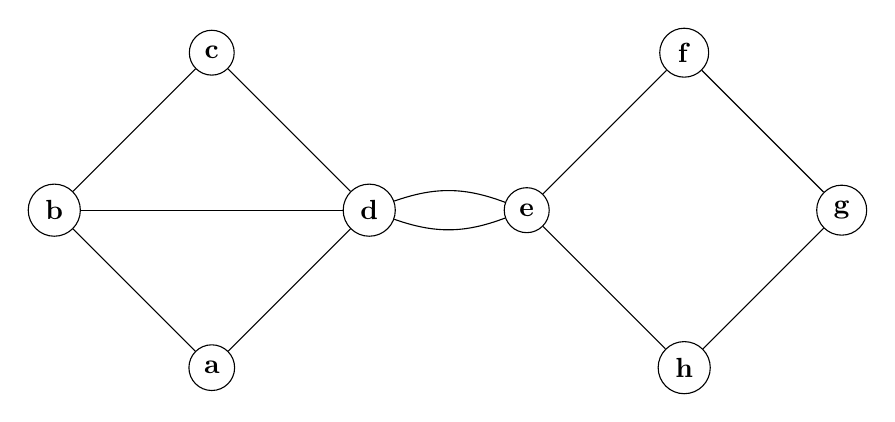
\begin{tikzpicture}[every loop/.style={}]
	
	\node[shape=circle,draw=black] (a) at (2, 0)     {\textbf{a}};
	\node[shape=circle,draw=black] (b) at (0, 2)     {\textbf{b}};
	\node[shape=circle,draw=black] (c) at (2, 4)     {\textbf{c}};
	\node[shape=circle,draw=black] (d) at (4, 2)     {\textbf{d}};
	\node[shape=circle,draw=black] (e) at (6, 2)     {\textbf{e}};
	\node[shape=circle,draw=black] (f) at (8, 4)     {\textbf{f}};
	\node[shape=circle,draw=black] (g) at (10, 2)     {\textbf{g}};
	\node[shape=circle,draw=black] (h) at (8, 0)     {\textbf{h}};
	
	
	\path[-] (b) edge (c);
	\path[-] (b) edge (a);
	\path[-] (b) edge (d);
	\path[-] (c) edge (d);
	\path[-] (a) edge (d);
	\path[-] (d) edge [bend left=20] (e);
	\path[-] (e) edge [bend left=20] (d);
	\path[-] (e) edge (f);
	\path[-] (e) edge (h);
	\path[-] (f) edge (g);
	\path[-] (h) edge (g);

	\end{tikzpicture} 
	\caption{Example for students to how to draw a undirected graph.}
	\label{g3}
\end{figure}

\begin{figure}[H]
	\centering
	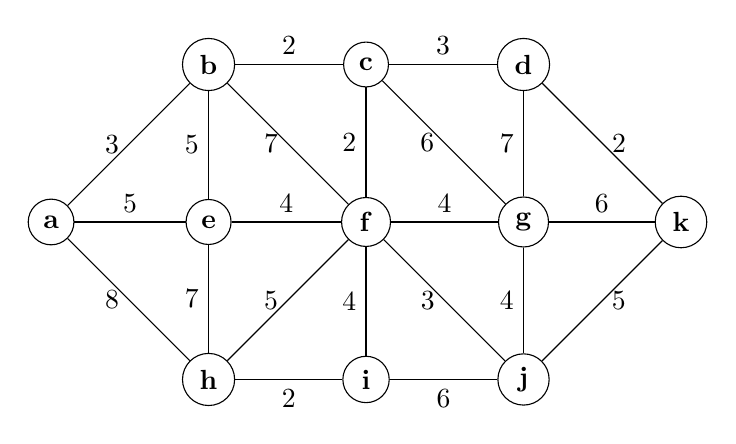
\begin{tikzpicture}
	\node[shape=circle,draw=black] (a) at (0, 2)     {\textbf{a}};
	\node[shape=circle,draw=black] (b) at (2, 4)     {\textbf{b}};
	\node[shape=circle,draw=black] (c) at (4, 4)     {\textbf{c}};
	\node[shape=circle,draw=black] (d) at (6, 4)     {\textbf{d}};
	\node[shape=circle,draw=black] (e) at (2, 2)     {\textbf{e}};
	\node[shape=circle,draw=black] (f) at (4, 2)     {\textbf{f}};
	\node[shape=circle,draw=black] (g) at (6, 2)     {\textbf{g}};
	\node[shape=circle,draw=black] (h) at (2, 0)     {\textbf{h}};
	\node[shape=circle,draw=black] (i) at (4, 0)     {\textbf{i}};
	\node[shape=circle,draw=black] (j) at (6, 0)     {\textbf{j}};
	\node[shape=circle,draw=black] (k) at (8, 2)     {\textbf{k}};

	\path[-] (a) edge node[left]{3} (b);
	\path[-] (a) edge node[above]{5} (e);
	\path[-] (a) edge node[left]{8} (h);
	\path[-] (b) edge node[left]{5} (e);
	\path[-] (b) edge node[left]{7} (f);
	\path[-] (b) edge node[above]{2} (c);
	\path[-] (e) edge node[above]{4} (f);
	\path[-] (e) edge node[left]{7} (h);
	\path[-] (h) edge node[left]{5} (f);	
	\path[-] (h) edge node[below]{2} (i);	
	\path[-] (c) edge node[above]{3} (d);
	\path[-] (c) edge node[left]{6} (g);
	\path[-] (c) edge node[left]{2} (f);
	\path[-] (f) edge node[above]{4} (g);
	\path[-] (f) edge node[left]{3} (j);
	\path[-] (f) edge node[left]{4} (i);
	\path[-] (i) edge node[below]{6} (j);	
	\path[-] (d) edge node[right]{2} (k);
	\path[-] (d) edge node[left]{7} (g);
	\path[-] (g) edge node[above]{6} (k);
	\path[-] (g) edge node[left]{4} (j);
	\path[-] (j) edge node[right]{5} (k);
		
	\end{tikzpicture} 
	\caption{Example for students to how to draw a weighted graph.}
	\label{g5}
\end{figure}

\end{document}

​

